%{{{ Preamble
\documentclass[usenatbib]{mnras}
\usepackage{graphicx}
\usepackage[export]{adjustbox}
\usepackage{bm}
\usepackage{amsmath}
\usepackage{amssymb}
\usepackage{algorithm}
\usepackage{algpseudocode}
\usepackage{subcaption}
\usepackage{layouts}
\usepackage{hyperref}
\usepackage[capitalise]{cleveref}
\usepackage{fancyvrb}
\usepackage{enumitem}
\usepackage{xcolor}
\usepackage[T1]{fontenc}
%}}}


\renewcommand\thesubsubsection{\Alph{subsubsection}.}
\newcommand{\nlive}{n_i}
\newcommand{\Like}{\mathcal{L}}
\newcommand{\DKL}{\mathcal{D}_\mathrm{KL}}
\newcommand{\logLmax}{\log \Like_\mathrm{max}}

\title[Approximating the end of nested sampling]{Approximating the end of nested sampling}
\author[Z. Hu et. al]{Zixiao Hu, Artyom Baryshnikov, Will Handley}

\begin{document}
\label{firstpage}
\pagerange{\pageref{firstpage}--\pageref{lastpage}}
\maketitle


\begin{abstract}
This paper develops a technique to estimate the runtime of nested sampling which works for any nested sampling implementation. At each iteration, the dimensionality of the current set of samples is inferred, then used to extrapolate the known likelihood profile using a Gaussian model function, which allows the remaining evidence and prior volume at termination to be calculated. The method finds the right order of magnitude at all times, obtaining the true endpoint within standard error generally around the halfway point, and converges to the true value by the end of the run.
\end{abstract}

\begin{keywords}
methods: data analysis -- methods: statistical
\end{keywords}

\section{Introduction}
Nested sampling is a multi-purpose algorithm invented by John Skilling which simultaneously functions as a probabilistic sampler, integrator and optimiser \citep{skilling}. It was immediately adopted for cosmology, and is now used in a wide range of physical sciences including particle physics, materials science \citep{physical_scientists} and machine learning \citep{sparse_reconstruction}. The core algorithm is unique in its estimation of volumes by \textit{counting}, which makes high-dimensional integration feasible. It also avoids problems faced by traditional Bayesian algorithms, such as multi-modality.
\par
The order of magnitude runtime of an algorithm, that is, whether termination is hours or weeks and months away, is of high importance to the end user. Currently, existing implementations of nested sampling (e.g. \citealt{multinest, polychord, ultranest}) either do not give an indication of runtime, or only provide crude measures of progress that do not directly correspond to the runtime. 
\par
This paper sets out a principled manner of endpoint estimation for nested sampling at each intermediate stage (as shown in \cref{fig:polychord_output}), the key idea being to use the existing samples to predict the likelihood in the region we have yet to sample from. We begin with an overview of nested sampling in \cref{sec:background}, followed by an examination of the anatomy of a nested sampling run to establish key concepts for endpoint prediction. \cref{sec:endpoint} then outlines the methodology we use, including discussion and comparisons to previous attempts. Finally, \cref{sec:results} presents the results and discussions for toy and cosmological chains, before we conclude.
\begin{figure}
\begin{Verbatim}[frame=single, commandchars=\\\{\}]
\textcolor{red}{Predicted endpoint: 25054 +/- 242}
\textcolor{red}{Progress: [=================>########] 72%}
___________________
lives      |   500 |
phantoms   | 24310 |
posteriors | 18018 |
equals     |   245 |
-------------------
ncluster   =  1/1
ndead      =  18018
nposterior =  18018
nequals    =  249
nlike      =  4159049
<nlike>    =  491.04 (9.82 per slice)
log(Z)     =  -12.55 +/- 0.27
\end{Verbatim}
\caption{Output from \textsc{PolyChord} for a typical nested sampling run. The predicted endpoint, shown in red, is calculated using the method described in this paper.}
\label{fig:polychord_output}
\end{figure}

\section{Background}\label{sec:background}
Let us begin with a brief description of the nested sampling algorithm to establish the necessary notation; for a more comprehensive treatment, we recommend Skilling's paper and the textbook \citet{sivia}. For a given likelihood $\mathcal{L}(\theta)$ and prior $\pi(\theta)$, nested sampling simultaneously calculates the Bayesian evidence
\begin{equation}\label{eq:evidence}
	\mathcal{Z} = \int \mathcal{L}(\theta)\pi(\theta)\ \mathrm{d}\theta
\end{equation}
while producing samples of the posterior distribution
\begin{equation}
	\mathcal{P}(\theta) = \frac{\mathcal{L}(\theta) \pi(\theta)}{\mathcal{Z}}.
\end{equation}
The algorithm operates by maintaining a set of $\nlive$ \textit{live points} sampled from the prior, which can vary in number throughout the run \citep{dynamic_ns}. At each iteration, the point with the lowest likelihood is removed and added to a list of \textit{dead points}. A new point is then drawn from the prior, subject to the constraint that it must have a higher likelihood than the latest dead point. Repeating the procedure leads to the live points shrinking around peaks in the likelihood.
\par
The integral in \eqref{eq:evidence} is then evaluated by transformation to a one-dimensional integral over the \textit{prior volume} $X$
\begin{equation}
	\mathcal{Z} = \int_0^1 \mathcal{L}(X)\ \mathrm{d}X \approx \frac{1}{2}\sum_{i=1} \mathcal{L}(X_{i-1}-X_{i+1}),
\end{equation}
where $X(\mathcal{L})$ is the fraction of the prior with a likelihood greater than $\mathcal{L}$. The prior volumes $X_i$ are unknown, but can be statistically estimated as follows: one can define a \textit{shrinkage factor} $t_i$ at each iteration $X_{i} = t_i X_{i-1}$, such that
\begin{equation}\label{eq:X_dist}
	X_i = \prod_{k=1}^i t_k.
\end{equation}
The $t_i$ are the maximum of $\nlive$ points drawn from $[0,1]$, so follow the distribution
\begin{equation}\label{eq:t_dist}
	P(t_i) = \nlive t_i^{\nlive-1}
\end{equation}
\begin{equation}\label{eq:t_moments}
    \langle\log t_i\rangle = -\frac{1}{\nlive}, \quad \mathrm{Var}(\log t_i) = \frac{1}{\nlive^2}.
\end{equation}
The algorithm terminates when an user-specified condition is met; a popular choice is to terminate when the evidence in the live points falls below some fraction $\epsilon$ of the accumulated evidence e.g. $10^{-3}$. The remaining live points are then killed off one by one without replacement and added to the evidence.
\par
Uncertainties in the evidence are dominated by the spread in the prior volume distribution, and the simplest way to estimate them is by Monte Carlo sampling over sets of $\bm{t}$. For any given problem, the uncertainty in $\log \mathcal{Z}$ is proportional to $1/\sqrt{\nlive}$, so $\nlive$ sets the resolution of the algorithm.

\section{The anatomy of a nested sampling run}
The following section aims to make an inventory of the information available to us at an intermediate iteration $i^{*}$, which we shall eventually use to make endpoint predictions. We present an anatomy of the progression of a nested sampling run in terms of the prior volume compression, the log-likelihood increase, the inferred temperature, and the dimensionality of the samples.

\subsection{Prior volume}
The key feature of nested sampling is that the sampling is controlled by prior volume compression. The task is to find the posterior typically lying in a tiny fraction of the prior volume, a total compression which is quantified by the average information gain, or \textit{Kullback-Leibler divergence}:
\begin{equation}\label{eq:DKL}
   \DKL = \int \mathcal{P}(\theta) \log \frac{\mathcal{P}(\theta)}{\pi(\theta)}\ \mathrm{d}\theta. 
\end{equation}
The bulk of the posterior lies within a prior volume $X = e^{-\DKL}$, which is the target compression. One gets there by iteratively taking steps of size $\Delta \log X_i = -1/n_i$, so that when we add up the contribution of each step in \eqref{eq:t_moments} we get
\begin{equation}
    \mathrm{E}(\log X_i) = -\sum_{k=1}^i \frac{1}{n_k}, \quad \mathrm{Var}(\log X_i) = \sum_{k=1}^i \frac{1}{n_k^2}.
\end{equation}
A constant step size in $\log X$ corresponds to a geometrically constant measure for the dead points (as shown in \cref{fig:dead_measure}), which is exactly needed to overcome the curse of dimensionality.
\begin{figure*}
\begin{center}
    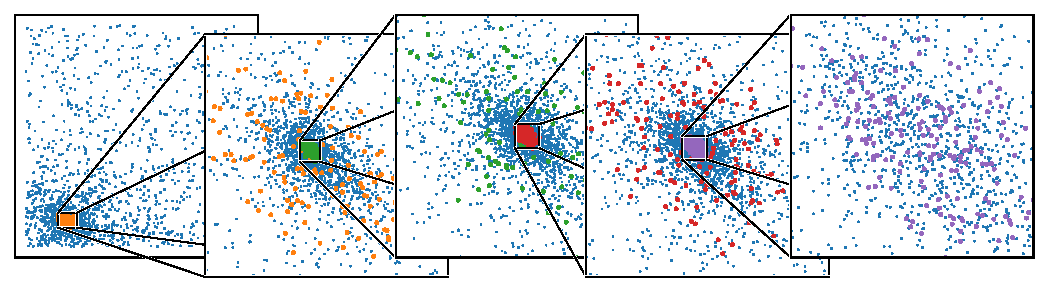
\includegraphics{figures/dead_measure_live.pdf}
\end{center}
\caption{The dead points of a nested sampling run, recursively zoomed in. Their density is constant in $\log X$, which is a geometrically constant measure $\propto \mathrm{d} V/V$, and hence scale invariant. The live points (larger dots) are uniform across the prior, plotted for comparison.}
\label{fig:dead_measure}
\end{figure*}
\par
The same is not true for the live points, which are uniformly distributed in prior volume. As a result, the maximum live point is found at 
\begin{equation}\label{eq:Xmin}
	\mathrm{E}(\log X_\mathrm{min}^{\mathrm{live}}) = \mathrm{E}(\log X_*) - \sum_{k=1}^{\nlive} \frac{1}{n_k} \approx -\frac{i_*}{\nlive} - \log \nlive - \gamma,
\end{equation}
with variance
\begin{equation}
	\mathrm{Var}(\log X_\mathrm{min}^{\mathrm{live}}) = \mathrm{Var}(\log X_*) + \sum_{k=1}^{\nlive} \frac{1}{n_k^2} \approx \frac{i_*}{\nlive^2} + \frac{\pi^2}{6}, 
\end{equation}
where the large $\nlive$ limit is taken for the approximation to the harmonic series, $\gamma$ being the Euler-Mascheroni constant.
\par
The live points therefore only get us a factor of $\log \nlive$ closer to the posterior bulk. In other words, it is not until we are around $\log \nlive$ away from $\log X = -\DKL$ that the samples look anything like the posterior. One can see from \eqref{eq:DKL} that the divergence increases linearly with dimension, so for large dimensionalities and typical live point numbers $\lesssim 1000$, this does not happen until near the end of the run.
Intuitively, it is because for a sharply peaked likelihood the live points are too diffuse to land there with any significant probability for most of the run.
\par
The above results are summarised in \cref{fig:logX_distribution}
\begin{figure*}
\begin{center}
    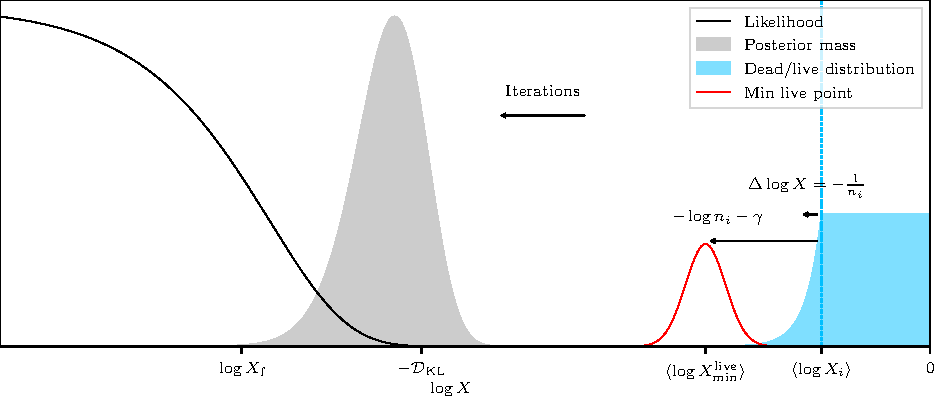
\includegraphics{figures/logX_distribution.pdf}
\end{center}
\caption{The distribution of the posterior mass in terms of $\log X$, the live points over the constrained prior and the smallest live point prior volume $\log X_\mathrm{min}^{\mathrm{live}}$ at an intermediate iteration $i_*$. For large values of $\DKL$ i.e. informative posteriors and/or large dimensionalities, the maximum live point is very far from the posterior bulk until the very end of the run. Note that the x-axis in this plot is $\log X$, so that the run proceeds from right to left to emphasise that the enclosed prior volume iteratively gets smaller. Plots of the sort from here onwards will be in terms of $-\log X$, where the run will more naturally proceed from left to right. }
\label{fig:logX_distribution}
\end{figure*}

\subsection{Log-likelihood}\label{sec:logL}
It is also useful to observe the distribution of the live and dead points in log-likelihood. We choose to examine a representative case of the $d$-dimensional multivariate Gaussian:
\begin{equation}\label{eq:gaussian_logL}
    \log \Like = \logLmax - X^{2/d}/2\sigma^2
\end{equation}
with maximum point $\logLmax$ and lengthscale $\sigma$ to get an insight into the analytics. The likelihood monotonically increases towards $\logLmax$, with the posterior samples eventually concentrated around the bulk at
\begin{equation}
    \langle\log\Like\rangle_\mathcal{P} = \log\mathcal{L}_\mathrm{max} - \frac{d}{2},  \quad \mathrm{Var}(\log\mathcal{L})_\mathcal{P} = \frac{d}{2}.
\end{equation}
We can again find the size of each step in log-likelihood, as well as the expected location of the maximum live point. Let us define a likelihood normalised by the distance to the maximum:
\begin{equation}
    y = \frac{\log\mathcal{L}-\log\mathcal{L}^*}{\log\mathcal{L}_\mathrm{max}-\log\mathcal{L}^*};
    \label{eq:normalised_likelihood}
\end{equation}
$y=0$ corresponds to the current point $\log\mathcal{L}^*$ and $y=1$ to the maximum $\log\mathcal{L}_\mathrm{max}$. At each iteration, $y$ increases by roughly
\begin{equation}
    \lim_{\nlive \to \infty}\Delta y \approx \frac{\mathrm{d} y}{\mathrm{d}\log X} \Delta \log X = \frac{2}{d \nlive}  
\end{equation}
in the large $\nlive$ limit. We can again sum the harmonic series to see that the maximum live point is expected to be at 
\begin{equation}
    y_{(\nlive)}^{\mathrm{live}} = \frac{2\log \nlive}{d},
\end{equation}
where we have used the notation of order statistics to denote the $x_{(n)}$ as the maximum of $n$ points. This is a very small fraction in high dimensions, showing again that until the end the live points are far from the posterior bulk, and certainly nowhere near the maximum.
\par
The above also implies that the normalised distance between the highest and second highest live point is roughly 
\begin{equation}
    y_{(\nlive)}^{\mathrm{live}} - y_{(\nlive - 1)}^{\mathrm{live}} \approx \frac{2}{d}.
\end{equation}
Before reaching the posterior bulk, $\logLmax - \log\Like^{*} > d/2$, so we must have
\begin{equation}
    \log \Like^{\mathrm{live}}_{(\nlive)} - \log \Like^\mathrm{live}_{(\nlive - 1)} > 1.
\end{equation}
In other words, the highest likelihood point is always at least an order of magnitude greater than the second highest. It is therefore typically the case that nearly all of the posterior mass is concentrated in a single point, the maximum live point, until the very end of the run when the prior volumes have shrunk enough to compensate.

\subsubsection*{Aside: nested sampling as a maximiser}
Previous literature \citep{Akrami_2010, Feroz_2011} has explored the potential for nested sampling to be used as a global maximiser, given its ability to handle multi-modalities. In particular, the latter authors emphasised that posterior samplers such as nested sampling find the bulk of the \textit{mass}, not the maximum of the distribution, but that this can be remedied by tightening the termination criterion. We now use the machinery we have developed to put this statement in more quantitative terms. 
\par
A more rigorous derivation (\cref{sec:logLmax}) shows that the maximum live point has mean and variance
\begin{equation}\label{eq:ylivemax}
	\lim_{d,\nlive\to\infty} y_\mathrm{max}^\mathrm{live} \sim \frac{2\log \nlive}{d} \pm \sqrt{\frac{2}{3}}\frac{\pi}{d}.
\end{equation}
Now let us take the dead point to be the termination point with likelihood $\log\Like_\mathrm{end}$ and prior volume $X_\mathrm{end}$, so that
\begin{equation}
	\epsilon = \frac{\int_0^{X_\mathrm{end}} \mathcal{L}\ \mathrm{d}X}{\int_0^\infty \mathcal{L}\ \mathrm{d}X}.
\end{equation}
Note that we have assumed that prior effects are negligible (so $1=\infty$), and that $\epsilon \ll 1$ so that the denominator is approximately the accumulated evidence. Computing this for \eqref{eq:gaussian_logL}, we find the answer in terms of lower incomplete gamma functions
\begin{equation}
\epsilon = 1- \frac{\Gamma_{d/2}\left(X_\mathrm{end}^{2/d}/2\sigma^2\right)}{\Gamma(d/2)}.
\end{equation}
Taking the $X_\mathrm{end}\ll (\sqrt{2}\sigma)^d$ limit (almost certainly valid at termination) we find
\begin{equation}
    \lim_{X_\mathrm{end}\ll (\sqrt{2}\sigma)^d} \epsilon \approx \frac{X_\mathrm{end}}{(\sqrt{2}\sigma)^d \ \Gamma(1+\frac{d}{2})} = \frac{(\log\mathcal{L}_\mathrm{max}-\log\mathcal{L}_\mathrm{end})^{\frac{d}{2}}}{\Gamma(1+\frac{d}{2})}.
\end{equation}
We thus have an expression relating $\mathcal{L}_\mathrm{end}$ at termination to the termination fraction $\epsilon$. This becomes yet more pleasing in the large $d$ limit, since $\epsilon^{2/d}\to 1$, we find via a Stirling approximation:
\begin{equation}
    \lim_{d\to\infty} \log\mathcal{L}_\mathrm{end} \approx \log\mathcal{L}_\mathrm{max} - \frac{d}{2e}.
\end{equation}
In the event that we keep $\epsilon$ in, we replace $\frac{d}{2e}\to \frac{d}{2e}\epsilon^{2/d}$, so we can of course battle the $\frac{d}{2e}$ term, but this becomes exponentially difficult in high dimensions.
\par
Putting this together, taking $\mathcal{L}_*$ in \eqref{eq:normalised_likelihood} to be $\mathcal{L}_\mathrm{end}$, and combining this with \eqref{eq:ylivemax} we find
\begin{equation}
    \boxed{
        \log{\mathcal{L}}_\mathrm{max}^\mathrm{live} \approx \log\mathcal{L}_\mathrm{max} - \frac{d}{2e} + \frac{\log n}{e} \pm \frac{\pi}{\sqrt{6}e}
    },
\end{equation}
showing that in general nested sampling will finish at a contour $d/2e$ away from the maximum log-likelihood. The final set of $n$ live points gets you $\log n/2e$ closer, with a chance of getting $\sim\pi/\sqrt{6}e=0.472$ closer still by statistical fluctuation. 
\par
A plot of the log-likelihood distribution at the end of a run is shown in \cref{fig:logL_distribution}
\begin{figure*}
\begin{center}
    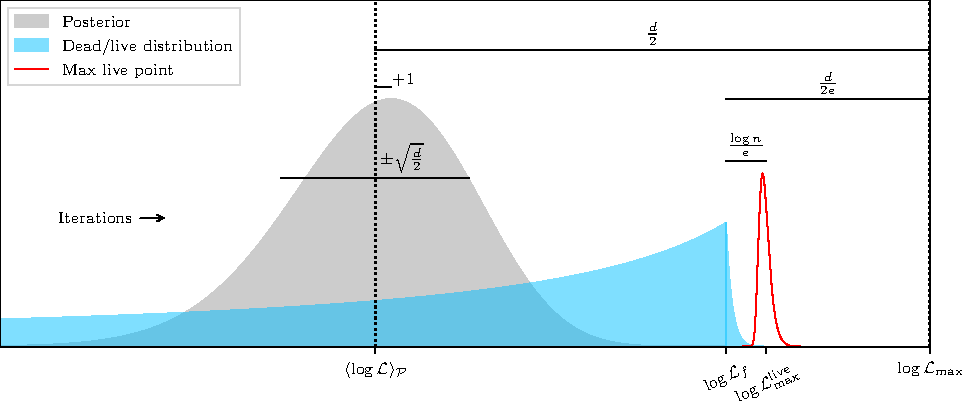
\includegraphics{figures/logL_distribution.pdf}
\end{center}
\caption{Distribution of samples as a function of $\log\mathcal{L}$, showing the posterior $\mathcal{P}(\log\mathcal{L})$, the distribution of the live points $\mathcal{\pi}(\log\mathcal{L} \mid \mathcal{L}>\mathcal{L}_*)$, and the distribution of the maximum likelihood live point $P(\log\mathcal{L}_\mathrm{max}^\mathrm{live})$. The distances are shown between these locations at the end of the run, the key takeaway being that in high dimensions the highest log-likelihood point of a nested sampling run is nowhere near the maximum in high dimensions.}
\label{fig:logL_distribution}
\end{figure*}


\subsection{Temperature}
\subsubsection*{Motivations}
As shown in the previous section, midway through the run nearly all of the posterior mass is concentrated at a single point. However, this does not capture the \textit{structure} of the posterior that has been explored and all of the information it provides. 
\par
We have the potential to fix this because nested sampling is invariant to monotonic transformations, so we can transform the likelihood as $\Like \to \Like^{\beta}$ without loss of information by trivially reweighting the samples. Increasing $\beta$ worsens the situation, while $\beta \to 0$ simply gives back the prior. There is, however, a significant intermediate range which makes the samples look like a posterior centred at the present contour, which will allow us to recover the structure of the samples. A schematic of the procedure is shown in \cref{fig:last_live_point}.
\par
\begin{figure}
\begin{center}
    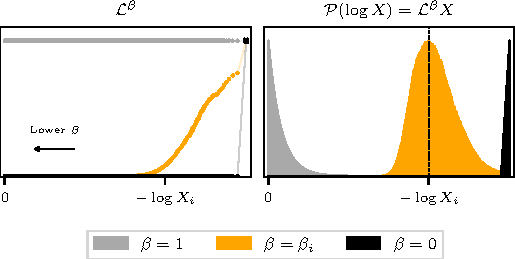
\includegraphics{figures/last_live_point.pdf}
\end{center}
\caption{The likelihood and posterior as a function of $\log X$ in the middle of a nested sampling run. Almost all of the posterior mass is concentrated at a single point with the highest compression, because it is orders of magnitude higher in likelihood. Reducing $\beta$ reweights to shift the posterior mass; taking $\beta \to 0$ goes too far and gives back the prior, but there is some intermediate $\beta = \beta^*$ which is significant because it centres the posterior at the current contour.}
\label{fig:last_live_point}
\end{figure}
\par
At this point it is relevant to note the correspondence between Bayesian inference and statistical mechanics, from which the above transform is derived. If one equates the parameters to microstates $i$, the negative log-likelihood to the microstate energy $E_i$, and the prior to the density of states $g_i$, then the posterior as given by the generalised Bayes' rule is the canonical ensemble
\begin{equation}
    p(E_i) = \frac{g_i e^{-\beta E_i}}{Z(\beta)} \quad \leftrightarrow \quad \mathcal{P}_\beta(\theta) = \frac{\mathcal{L}^{\beta}(\theta)\pi(\theta)}{\mathcal{Z}(\beta)}
\end{equation}
at the inverse temperature $\beta = 1/T$. As noted by \citet{demons}, thermal algorithms such as thermodynamic integration \citep{path_sampling} get the evidence by evolving through a series of canonical ensembles via some temperature schedule, but nested sampling instead maintains \textit{microcanonical} ensembles, which are the iso-likelihood contours. Each step moves at constant relative volume entropy $\Delta \log X$, which allows the algorithm to handle phase transitions \citep{statmech}. 
\par
Because the temperature of a microcanonical ensemble is a derived property rather than a parameter, there is some freedom in its definition. Returning to our original motivation, we make the connection that the temperature is the reweighting $\Like \to \Like^{\beta}$ which centers the ensemble around the current energy. We now present several temperatures that achieve this aim, each of which one can plausibly consider to be the current temperature of a nested sampling run.

\subsubsection{Microcanonical temperature}
The obvious candidate is the microcanonical temperature $\partial S/\partial E$, where the volume entropy is $\log X$ and the energy is as usual $-\log \Like$. This gives the density of states; as discussed in Skilling's original paper,
\begin{equation}
    \beta_\mathrm{M}  = - \frac{\mathrm{d} \log X}{\mathrm{d} \log \Like} \Bigg\vert_{\log \Like^{*}}.
\end{equation}
is the $\beta$ at which $\Like^{\beta} X$ peaks at $\log X^{*}$, if we assume differentiability, which is exactly the intuition we were aiming for to put the ensemble bulk at the current contour.
Its value can be easily obtained via finite difference of the $\log \Like$ and $\log X$ intervals, albeit subject to an arbitrary window size for the differencing (in practice, we find that above a threshold of around 10 iterations the result is fairly insensitive to this choice). 
\par
The ensemble bulk can be placed at the current point in several other plausible ways, which are discussed below.

\subsubsection{Canonical temperature}
Another temperature considered by Habeck is that at which the current energy (i.e. $-\log \Like^{*}$) is the average energy of the entire ensemble. One can obtain it by inverting 
\begin{equation}
    \langle \log \Like \rangle_{\mathcal{P}_\beta} = \log \Like^{*}
\end{equation}
to get the `canonical' temperature $\beta_\mathrm{C}$. While $\beta_\mathrm{M}$ is derived from (the gradient of) a single contour, this temperature uses the entire ensemble. It has the desirable property that it rises monotonically with compression, in analogy to a monotonic annealing schedule.

\subsubsection{Bayesian temperature}
We furthermore propose a temperature $\beta_\mathrm{B}$ that is obtained via Bayesian inference, which returns a distribution rather than a point estimate. Since each value of $\beta$ leads to a different likelihood $\Like^{\beta}$, one can consider the posterior distribution as a function of $\log X$ to be \textit{conditioned} on $\beta$. We can therefore write
\begin{equation}
   \mathcal{P}(\log X \mid \beta) = \frac{\Like^{\beta}(X) X}{\mathcal{Z(\beta)}}.
\end{equation}
What we would really like is the distribution of $\beta$ at the present iteration, so the natural step is to invert this via Bayes' rule;
\begin{equation}
    P\left(\beta \mid \log X^{*}\right) = \frac{\mathcal{P}\left(\log X^{*} \mid \beta\right) P\left(\beta\right)}{P\left(\log X\right)}.
\end{equation}
As with all Bayesian analyses, the distribution of $\beta$ is fixed up to a prior, which we choose to be uniform in $\beta$. The obtained temperatures are consistent with the previous two choices, which may seem oddly coincidental. However, closer inspection reveals that large values of $P(\beta \mid \log X^{*})$ are the temperatures with a large value of the posterior at the present contour, normalised by the corresponding evidence. Thus the Bayesian temperature uses the same idea as the microcanonical one, except it accounts for the spread in the result.

\subsubsection*{Comparisons}
\cref{fig:beta_comparison} shows the three temperatures as a function of compression for two cases, one containing a phase transition and one without. They are consistent in both cases when there is a single dominant phase, but differ during a phase transition. The canonical temperature is the only one that rises monotonically with compression.
\begin{figure}
\begin{center}
    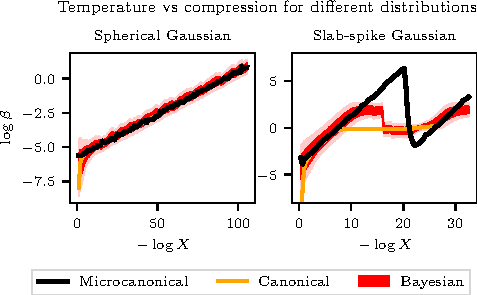
\includegraphics{figures/beta_comparison.pdf}
\end{center}
\caption{Inferred temperatures using the microcanonical, canonical and Bayesian definitions. All are consistent for a single phase, but differ during a phase transition.}
\label{fig:beta_comparison}
\end{figure}
\par
One should keep in mind that despite the above theoretical reasoning, our introduction of the likelihood transformation was ultimately motivated by our wish to utilise the extra degree of freedom it provides. As we will see below, we recommend choosing the exact definition depending on what is useful for the transformation to do. 

\subsection{Dimensionality}
We can immediately use the inferred temperature to track how the effective dimensionality of the posterior changes throughout the run, which was previously inaccessible. \citet{Handley_2019} demonstrated that at the end of a run, a measure of the number of constrained parameters is given by the Bayesian model dimensionality (BMD), defined as the posterior variance of the information content:
\begin{equation}
\frac{d_G}{2} = \int \mathcal{P}(\theta) \left(\log \frac{\mathcal{P}(\theta)}{\pi(\theta)} - \DKL\right)^2 \: \mathrm{d}\theta
= \langle \mathcal{I}^2 \rangle_\mathcal{P} - \langle \mathcal{I} \rangle^2_\mathcal{P}.
\end{equation}
\par
Calculating the quantity using intermediate set of weighted samples (which is concentrated at a single point) leads to vanishing variance, hence also dimensionality. However, we can recover the structure of the posterior together with the true dimensionality by adjusting the temperature. Dimensionality estimates are plotted in \cref{fig:d_G_spherical} for a spherical 32-d Gaussian, for which the true dimensionality is known. 
\par
The different choices of temperature are again consistent, but for the rest of this paper we choose the Bayesian $\beta$, because it provides a better reflection of the uncertainty in the estimate; the others, while fluctuating around the true value, are often many standard errors away from the true value at each single point.
\begin{figure}
\begin{center}
    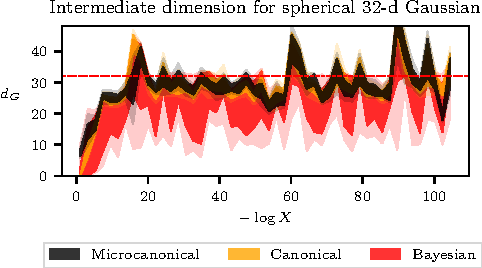
\includegraphics{figures/d_G_spherical.pdf}
\end{center}
\caption{Dimensionality estimates using the different temperatures for a spherical 32-d Gaussian. Again, all are consistent, but the Bayesian definition has a uncertainty which includes the true value far more consistently than for the other definitions.}
\label{fig:d_G_spherical}
\end{figure}

\subsubsection*{Anisotropic compression}\label{sec:elongated}
Plots of samples dimensionality against compression also draw attention to the \textit{directions} in which the samples are constrained throughout the run. As a concrete example, consider an elongated Gaussian in a unit hypercube prior with $\mu = \bm{0}$ and $\Sigma = \mathrm{diag}\left(10^{-3}, 10^{-3}, 10^{-3}, 10^{-6}, 10^{-6}, 10^{-6}\right)$, for which the dimensionality estimates are plotted in \cref{fig:d_G_elongated}. Alongside is a view of the distribution of live points across the prior for two directions with different scales, which shows the level to which those parameters have been constrained at different times.
\par
A feature of nested sampling made apparent here is that parameters with high variance are initially `hidden'. Compression occurs in the direction which is most likely to have a sample of higher likelihood, and initially it is much easier to find a better point along the direction of a parameter that is poorly constrained. Lower variance parameters are constrained much later, and before that happens it appears as though those parameters have a uniform distribution.
\begin{figure}
\begin{center}
    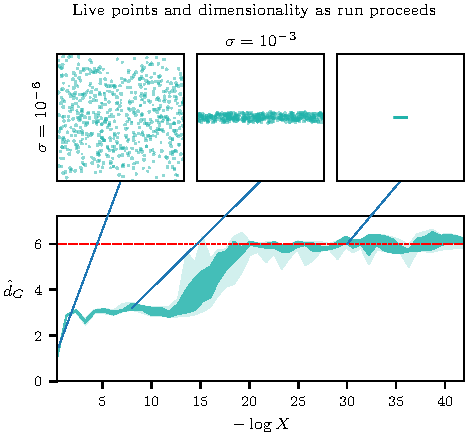
\includegraphics{figures/d_G_elongated.pdf}
\end{center}
\caption{Dimensionality estimates for a Gaussian that is elongated in half of its dimensions. The locations of the live points in the prior are shown at three stages, indicated by the vertical lines. As can be seen from the live point distribution, the prior does not compress in the higher variance direction until much later in the run, and early on it appears as if those directions are completely unconstrained.}
\label{fig:d_G_elongated}
\end{figure}
\par
It is important to appreciate that at lower compressions the samples truly lie in a lower-dimensional space, rather than some artefact of the way we view them. Anticipating the full dimensionality of the space is therefore just as impossible as that associated with a slab-spike geometry, so in this sense such geometries contain a `compressive phase transition'. 

\section{Endpoint prediction}\label{sec:endpoint}
The time complexity of nested sampling \citep{supernest} is
\begin{equation}
    T \propto \nlive \times \langle \mathcal{T}\{ \Like(\theta) \} \rangle \times \langle f_\mathrm{sampler} \rangle \times \DKL.
\end{equation}
The second term is the relatively constant time per likelihood evaluation. The third is the average number of evaluations required to replace a dead point with a live point at higher likelihood, which is given by the implementation and usually does not vary in orders of magnitude. The primary unknown during a run, and therefore our primary interest, is the final term: the compression required to get from prior to posterior. 
\par
Further exploration can be found in the talk [\citenum{kcl_talk}] and the upcoming paper \citet{scaling_frontier}.

\subsection{The termination prior volume}
To be exact, one wishes to find the compression factor $\log X_ \mathrm{f}$ at which the termination criterion is met, which is larger in magnitude than $\DKL$ (\cref{fig:logX_distribution}). The problem is that at an intermediate iteration we only know the posterior up to the maximum log-likelihood live point, which until just before the end is quite far from the posterior bulk. 
\par
In order to get an idea of where the true posterior bulk sits, we need to predict what the posterior looks like past the highest live point. We do this by \textit{extrapolating} the known likelihood profile; that is, the trajectory of $\Like(X)$ traced out by the live and dead points. 
\par
One would never use this predicted posterior to do inference, since more accuracy can always be achieved by simply finishing the run. However, it is more than sufficient for making a prediction for $\log X_\mathrm{f}$. Quantitatively, this proceeds as follows: fit a function $f(X, \phi)$  with some parameters $\phi$ to the known likelihood profile, which allows us to express the prior volume we need to compress to as
\begin{equation}
	\Delta \mathcal{Z} = \epsilon \mathcal{Z}_\mathrm{tot},
\end{equation}
\begin{equation}\label{endpoint}
	\int_0^{X_\mathrm{f}} f(X, \phi)\ \mathrm{d}X = \epsilon \left( \int_0^{X_i} f(X, \phi)\ \mathrm{d}X + \mathcal{Z}_\mathrm{dead} \right),
\end{equation}
where $X_i$ is the volume of the iteration we have currently compressed to, and $\mathcal{Z}_\mathrm{dead}$ is the evidence we have accumulated up to this point. $X_\mathrm{f}$ can then be identified by solving the above equation either analytically or numerically. 
\par
Once $X_\mathrm{f}$ is known, the corresponding iteration count depends on the live point schedule. The conversion is easiest in the constant $\nlive$ case; at each iteration $\log X$ decreases by $1/n$, so the total number of iterations $N_\mathrm{f}$ will be
\begin{equation}
	N_\mathrm{f} = - n\log X_\mathrm{f} .
\end{equation}


\subsection{How to extrapolate?}
A key observation is that the Bayesian model dimensionality is the equivalent dimension of the posterior if it were actually Gaussian. Fitting a Gaussian of this dimension to the likelihood profile therefore makes a reasonable approximation to the true distribution, without explicitly assuming the form of the likelihood function. The parameterisation of the Gaussian that we fit is the same as that given in \cref{sec:logL}, which we shall repeat here for clarity;
\begin{equation}\label{gaussian}
    f(X; \phi) = \logLmax - X^{2/d}/2\sigma^2
\end{equation}
The extrapolation then proceeds thus:
\begin{enumerate}[leftmargin=*]
    \item Find the current dimensionality ${d}_G^{*}$ of the posterior at the Bayesian temperature
    \item Take the live point profile and do a least squares fit to \eqref{gaussian}, stipulating that $d = {d}_G^{*}$ to infer $\logLmax$ and $\sigma$ 
    \item Use the likelihood predicted by these parameters to solve \eqref{endpoint} for $X_\mathrm{f}$
\end{enumerate}
The advantage of fitting a Gaussian is that the procedure can be sped up analytically. Firstly, the least squares regression is trivial because analytic estimators exist; the cost function 
\begin{equation}\label{chi squared}
	C^2(\logLmax, \sigma) = \sum_i \left| \log \Like_i - f(X_i; \logLmax, \sigma) \right| ^2
\end{equation}
is minimised with respect to $(\logLmax, \sigma)$ when
\begin{equation}\label{eq:sigma}
    \sigma^2 = \frac{N \sum_i X_i^{4/d} - \left(\sum_i X_i^{2/d}\right)^2}{2 \sum_i \log \Like_i \sum_i X_i^{2/d} - 2N \sum_i X_i^{2/d}\log \Like_i },
\end{equation}
and
\begin{equation}\label{eq:logLmax}
    \logLmax = \frac{1}{N} \sum_i \log \mathcal{L}_i + \frac{1}{2N\sigma^2} \sum_i X_i^{2/d}.
\end{equation}
Secondly, the termination prior volume can also be obtained analytically. Rewriting \cref{endpoint} in terms of the Gaussian parameters gives
\begin{equation}
	\epsilon = \frac{\int_0^{X_\mathrm{f}} \Like_\mathrm{max} \exp\left(-X^{2/d}/2\sigma^2\right)\ \mathrm{d}X}{\int_0^{X_i} \Like_\mathrm{max} \exp\left(-X^{2/d}/2\sigma^2\right)\ \mathrm{d}X + \mathcal{Z}_\mathrm{dead}}.
\end{equation}
The integrals have the analytic solution
\begin{equation}
	\int_0^{X_k} \Like_\mathrm{max} \exp\left(-X^{2/d}/2\sigma^2\right)\ \mathrm{d}X = \frac{d}{2} \cdot \left(\sqrt{2}\sigma\right)^d \cdot \gamma_k
\end{equation}
where $\gamma_k = \Gamma_{d/2}\left(X_k^{2/d}/2\sigma^2\right)$ is the lower incomplete gamma function. After taking the inverse of  $\gamma$ and a few more steps of algebra, we arrive at
\begin{equation}
    \log X_\mathrm{f} = \frac{d}{2}\log 2\sigma^2	+ \log \Gamma^{-1}_{d/2} \left(\epsilon \gamma_i+ \frac{\epsilon\mathcal{Z}_\mathrm{dead}}{ \left( 2\sigma^2 \right)^{d/2}\Like_\mathrm{max}}\right),
\end{equation}
and $N_\mathrm{f}$ is of course just $-\nlive$ multiplied by this. Intuitively, the above procedure can be thought of as inferring the number of constrained parameters, then extrapolating them up to find the point at which they will be fully constrained. 
\par
One might wonder why we do not obtain $d$ via least squares regression together with the other parameters; extensive testing has shown it to be far less stable.

\subsection{Alternative approaches}
We consider here several alternative approaches to endpoint estimation to compare against our method. 
\subsubsection{Integral progress}
One alternative approach, used in \textsc{Ultranest} \citep{ultranest}, derives a progress bar based on the fraction of the accumulated integral compared to the remaining integral, approximated as 
\begin{equation}\label{eq:integral_progress}
    \mathcal{Z}_\mathrm{rem} \approx \Like_\mathrm{max}^{\mathrm{live}} X^{*}.
\end{equation}
There are a few problems here. Firstly, runtime is proportional to compression rather than accumulation of the integral, since it takes just as long to traverse the width of the bulk as it does any other width. Secondly, because of the point-like nature of the posterior mid-run, the remaining integral approximated as such holds nearly all of the evidence, so the relative fraction of the accumulated and remaining evidence is simply be zero for most of the run. Furthermore, approximation \eqref{eq:integral_progress} is always an underestimate, because as previously found the maximum live point is generally nowhere near the true maximum.
\par
This approach can be useful in low dimensions when the live points are always near the maximum, but in general is less reliable.

\subsubsection{Extrapolating evidence increments}
Seasoned users of nested sampling might be curious how the method compares to simply extrapolating the increments of evidence to roughly estimate when the evidence converges. We do this for a spherical Gaussian and compare it to our method. At an intermediate stage of the run, the most recent outputs might look something like that shown in the first two columns of the table in \cref{fig:inc_extrapolate}. Extrapolating those data to a linear and exponential profile yields endpoint estimates plotted in the graph to the right. 
\par
The linear extrapolation is clearly an underestimate, since it fails to account for the long tail of the nonlinear profile. The increments are also not quite exponential, since the exponential fit leads to a large overprediction. The predicted endpoint over the course of a run for $d = 16$, $\sigma = 0.01$, as shown in \cref{fig:inc_predictions}, shows the same result. One might expect an average to be more accurate, but this tends to be biased towards the exponential prediction, and there is no obvious choice of weighting that would fix this.
\par
More importantly, we find that for real likelihoods which have an element of noise the extrapolation often diverges, for instance when the increments do not monotonically decrease. Directly extrapolating the evidence increments is therefore far less stable than the previous method, and generally not a reliable method for prediction.
\begin{figure}
\begin{adjustbox}{valign=t, scale=0.72}
\subfloat{\begin{tabular}{|c|c|c|}
\hline
iteration & log Z  & $\Delta\log Z$   \\
\hline
5000 & -1435.8 & 190.8 \\
5500 & -1264.6 & 171.2 \\
6000 & -1123.7 & 140.9 \\
6500 & -991.5 & 132.2 \\
7000 & -885.0 & 106.6 \\
7500 & -790.3 & 94.7 \\
8000 & -702.6 & 87.7 \\
8500 & -619.7 & 82.9 \\
9000 & -551.8 & 67.9 \\
9500 & -492.7 & 59.1 \\
\hline
\end{tabular}}
\end{adjustbox}
\quad
\begin{adjustbox}{valign=t}
\subfloat{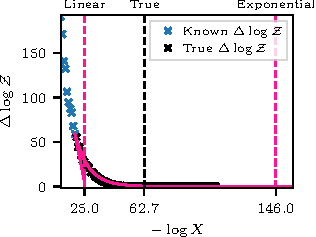
\includegraphics{figures/inc_extrapolate.pdf}}
\end{adjustbox}
\caption{Extrapolating the increments of evidence. The left column shows the output of a nested sampling run, and the right column shows the extrapolation.}
\label{fig:inc_extrapolate}
\end{figure}
\begin{figure}
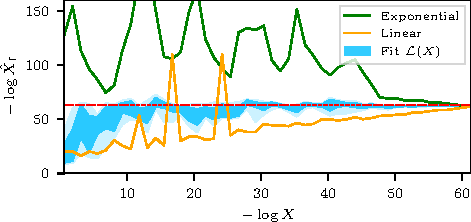
\includegraphics{figures/inc_predictions.pdf}
\caption{Endpoint predictions for a spherical Gaussian. Extrapolating the evidence increments in a linear/exponential manner under/overpredicts the endpoint, both of which do considerably worse than the method of extrapolating the likelihood.}
\label{fig:inc_predictions}
\end{figure}

\section{Results}\label{sec:results}
Now that we have a method for predicting the endpoint, it can be tested on a range of distributions. We begin by considering a series of toy examples to explore the capabilities and limitations of the method, before presenting results for real cosmological chains.
\subsection{Toy examples}
\subsubsection{Gaussians}
Predictions for spherical Gaussians of various dimensions are shown in \cref{fig:gauss_predictions} as a benchmark for when fitting a Gaussian distribution is exact. All were run with $\nlive = 500$ except for one $\nlive=2000$ for comparison, with each Gaussian having a width of $\sigma = 0.01$. The correct endpoint is recovered to within standard error at all points except the very beginning, when the parameters have hardly been constrained. 
\par
We note that as with nested sampling in general, increasing $\nlive$ improves the resolution and reliability of the inferences, which can be seen from the middle two plots.
\begin{figure*}
\begin{center}
    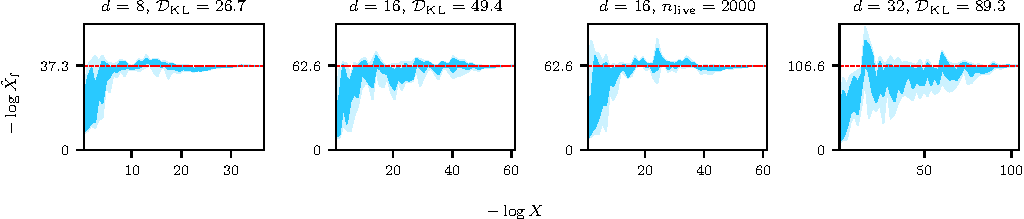
\includegraphics{figures/gauss_predictions.pdf}
\end{center}
\caption{Endpoint predictions for a spherical Gaussian run with $\nlive=500$ (except for the third plot from left). The correct endpoint is obtained for all but the earliest iterations, and the uncertainty is controlled by the number of live points, which can be seen from the two $d = 16$ plots.}
\label{fig:gauss_predictions}
\end{figure*}
We also observe the effect of elongating the Gaussian, using the same example as \cref{sec:elongated}. \cref{fig:elongated_logXfs} shows a step-like trend similar to the inferred dimensionalities, reflecting the fact that the full dimensionality is undetectable at lower compression factors. The endpoint for a likelihood whose remaining three directions are completely unconstrained coincides with our predictions at early iterations, showing that the two cases are indistinguishable. 
\begin{figure*}
\begin{center}
    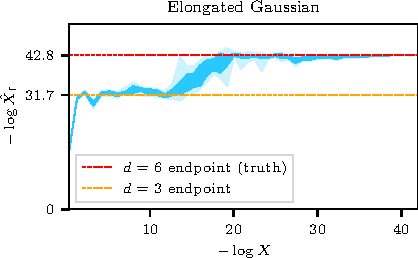
\includegraphics{figures/elongated_logXfs}
\end{center}
\caption{Endpoint prediction for an elongated Gaussian. At early stages, the full dimensionality is undetectable, and the endpoint is predicted to be the same as for a likelihood with three unconstrained directions. Only once the prior has been compressed enough to constrain the other three directions does the prediction converge to the true value.}
\label{fig:elongated_logXfs}
\end{figure*}

\subsubsection{Cauchy}
One case that might be expected to cause problems is the pathological Cauchy distribution, which is far from a Gaussian. \cref{fig:cauchy_predictions} shows the predictions for a likelihood of the form
\begin{equation}
	\log\mathcal{L} = \log\mathcal{L}_\mathrm{max} - \frac{1 + d}{2} \log \left(1 + \frac{X^2}{\gamma^2}\right),
\end{equation}
choosing $d = 10$ and allowing $\gamma$ to vary. The correct estimate is obtained to within standard error by about halfway, but before that is quite off. The key limitation is that the estimate is wrong early on not because the compression is anisotropic, or that there is a phase transition; rather, it is a limitation of the reducing the likelihood to a Gaussian via the BMD, which is itself less stable for a Cauchy.
\par
However, the right order of magnitude is obtained at all times, so this is not a major concern. The Cauchy is also a pathological case, and the same problem does not rear its head in more realistic cases, as we shall see next.
\begin{figure*}
\begin{center}
    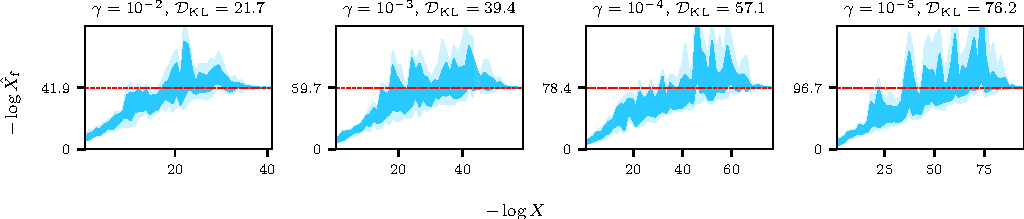
\includegraphics{figures/cauchy_predictions.pdf}
\end{center}
\caption{Predictions for the Cauchy distribution for various widths $\gamma$ and $\nlive = 500$. The endpoint is underestimated for the first half of the run, but this is a limitation of the Gaussian approximation rather than a lack of information mid-run.}

\label{fig:cauchy_predictions}
\end{figure*}

\subsection{Cosmological examples}
Finally, we evaluate the method on real cosmological chains. \cref{fig:lcdm_logXfs} presents the endpoints (calculated after the fact) for nested sampling runs for curvature quantification on several common cosmological datasets (details in \citet{curvature_tension}). 
\par
The \textsc{SH0ES}, \textsc{BAO} and \textsc{lensing} chains are `easy' low $\DKL$ inferences, so it is expected that the correct endpoint is inferred practically from the start. The \textsc{Planck} endpoints, on the other hand, are not correct until at least midway through. However, this is expected from the covariance of the \textsc{Planck} likelihood, which consists of principal components of many scales and therefore elongated in many dimensions. It is therefore of the same class as the elongated Gaussian presented in \cref{sec:elongated}; the samples exist in a lower dimensional subspace mid-run, which slowly increases to the full dimensionality only at the end of the run.
\begin{figure*}
\begin{center}
    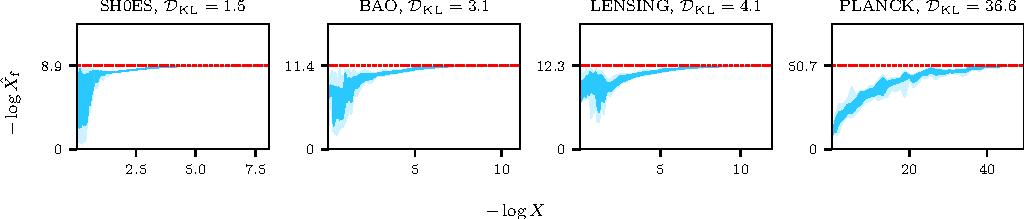
\includegraphics{figures/lcdm_logXfs.pdf}
\end{center}
\caption{Endpoint predictions for cosmological likelihoods. The first three low $\DKL$ inferences get the correct endpoint from the start, while the \textsc{Planck} chain takes longer to converge because the likelihood is highly covariant and thus subject to anisotropic compression, which makes the samples lie in a lower dimensional subspace mid-run.}
\label{fig:lcdm_logXfs}
\end{figure*}


\section{Conclusion}
We have presented a method for predicting the endpoint of a nested sampling run, by inferring the Bayesian model dimensionality of a set of samples mid-run and using it to extrapolate the known likelihood profile. 
\par
The method in general converges to the correct endpoint by about the halfway point, and gets the correct order of magnitude throughout. Consistent predictions are obtained for both toy and cosmological examples. The accuracy is typically limited by the information available mid-run, either because of a phase transition or because the anisotropy of the nested sampling compression. Pathological distributions, such as a Cauchy, lead to less stable inferences of the dimensionality and expose the limitations of a Gaussian approximation, though the order of magnitude is still correct.  
\par
Further work can be done to experiment with more flexible basis functions for regression of the likelihood profile, so that it is less dependent on the Gaussian approximation.

\appendix
\section{The maximum live log-likelihood}\label{sec:logLmax}
Assume a Gaussian likelihood
\begin{equation}\label{eq:logL}
	\log\mathcal{L} = \log\mathcal{L}_\mathrm{max} - X^{2/d}/2\sigma^2.
\end{equation}
The distribution of the true posterior in $\log\mathcal{L}$ is
\begin{equation}
    P(\log\mathcal{L}) = \frac{1}{\Gamma\left(\frac{d}{2}\right)}e^{\log\mathcal{L}-\log\mathcal{L}_\mathrm{max}} (\log\mathcal{L}_\mathrm{max}-\log\mathcal{L})^{\frac{d}{2}-1}
\end{equation}
i.e. $2(\log\mathcal{L}_\mathrm{max}-\log\mathcal{L}) \sim \chi^2_{d}$. The posterior average and variance of $\log \mathcal{L}$ are given by
\begin{equation}
    \langle\log\mathcal{L}\rangle_\mathcal{P} = \log\mathcal{L}_\mathrm{max} - \frac{d}{2},  \quad \mathrm{Var}(\log\mathcal{L})_\mathcal{P} = \frac{d}{2}.
\end{equation}
Meanwhile, the live points are uniformly distributed over the constrained prior and hence have probability distribution
\begin{multline}
	P(\log\mathcal{L}) = \frac{d}{2}\frac{(\log\mathcal{L}_\mathrm{max}-\log\mathcal{L})^{\frac{d}{2}-1}}{(\log\mathcal{L}_\mathrm{max}-\log\mathcal{L}_*)^{\frac{d}{2}}} \\
    [\log\mathcal{L}_* < \log\mathcal{L} <\log\mathcal{L}_\mathrm{max}],
    \label{eq:PL}
\end{multline}
It is helpful at this stage to define a parameter
\begin{equation}
    y = \frac{\log\mathcal{L}-\log\mathcal{L}_*}{\log\mathcal{L}_\mathrm{max}-\log\mathcal{L}_*}
    \label{eq:y}
\end{equation}
as a normalised measure of how far a point is between the latest dead point and the maximum log-likelihood, with $y=0$ corresponding to $\mathcal{L}_*$ and $y=1$ to $\mathcal{L}_\mathrm{max}$, so that
\begin{equation}
    P(y) = \frac{d}{2}(1-y)^{\frac{d}{2}-1} \quad [0<y<1].
    \label{eq:Py}
\end{equation}
We now seek the distribution for the maximum likelihood of the live points, $\log\mathcal{L}_\mathrm{max}^{\mathrm{live}}$. Using the result that the maximum of $n$ variables with cumulative distribution $F(y)$ follows $\frac{d}{dy}( 1- (1-F(y))^n)$, we obtain
\begin{multline}
    P(y_\mathrm{max}^\mathrm{live}) = \frac{nd}{2}(1-y_\mathrm{max}^\mathrm{live})^{\frac{d}{2}-1}\left(1-(1-y_\mathrm{max}^\mathrm{live})^{\frac{d}{2}}\right)^{n-1}\\ 
    [0<y_\mathrm{max}^\mathrm{live}<1],
    \label{eq:Pyhat}
\end{multline}
which may be roughly summarised as
\begin{multline}
    y_\mathrm{max}^\mathrm{live} \sim 1-\frac{\Gamma(1+\frac{2}{d})\Gamma(1+n)}{\Gamma(1+\frac{2}{d}+n)} \\
     \pm \left( \frac{\Gamma(1+n)\Gamma(1+\frac{4}{d})}{\Gamma(1+\frac{4}{d}+n)} - \frac{\Gamma(1+\frac{2}{d})^2 \Gamma(1+n)^2}{\Gamma(1+\frac{2}{d}+n)^2}\right)^{\frac{1}{2}},
    \label{eq:ymax}
\end{multline}
or in the large $d$, $n$ limit
\begin{align}
    \lim_{d\to\infty} y_\mathrm{max}^\mathrm{live} &\sim \frac{2H_n}{d} \pm \left(\frac{2(\pi^2 - 6\Psi^{(1)}(1+n))}{3d^2}\right)^{\frac{1}{2}},
    \label{eq:ymaxd}\\
    \lim_{d,n\to\infty} y_\mathrm{max}^\mathrm{live} &\sim \frac{2\log n}{d} \pm \sqrt{\frac{2}{3}}\frac{\pi}{d},
    \label{eq:ymaxdn}
\end{align}
where $\psi^{(1)}$ is the trigamma function and $H_n$ is the $n$th harmonic number.
\par
This shows that in general the live points are nowhere near the maximum log-likelihood at any iteration, though they do steadily squeeze the interval $[\log\mathcal{L}_*,\log\mathcal{L}_\mathrm{max}]$. In particular, in high dimensions $n$ only gets us harmonically/logarithmically closer, whilst $d$ pushes us linearly further away.

\bibliographystyle{mnras}
\bibliography{references}

\label{lastpage}
\end{document}

